% !TeX encoding = UTF-8
% !TeX spellcheck = ru_RU
\documentclass[a4paper,14pt]{extarticle} %размер бумаги устанавливаем А4, шрифт 14пунктов
\usepackage{amssymb,amsfonts,amsmath,mathtext,cite,enumerate,float} %подключаем нужные пакеты расширений
\usepackage[T2A, T1]{fontenc}
\usepackage{cmap}
\usepackage[utf8]{inputenc}%включаем свою кодировку: koi8-r или utf8 в UNIX, cp1251 в Windows
\usepackage[english, russian]{babel}%используем русский и английский языки с переносами

\usepackage{graphicx} %хотим вставлять в диплом рисунки?
\graphicspath{{img/}}%путь к рисункам

\usepackage[colorlinks=false,pdfborder={0 0 0}]{hyperref} %использование гиперссылок, colorlinks - цвет текста ссылки, pdfborder - окантовка. 

%шрифт Times New Roman
%\usepackage{fontspec}
%\setmainfont{Times New Roman}
%\setallmainfonts{Times New Roman}

\usepackage{titlesec}
\titleformat{\section}[block]
{\filcenter\large}
{\thesection}
{1em}{\MakeUppercase}
\titlespacing*{\section}{0pt}{-30pt}{*4}

\makeatletter
%\renewcommand{\@biblabel}[1]{#1.} % Заменяем библиографию с квадратных скобок на точку:
\makeatother


\usepackage{geometry} % Меняем поля страницы
\geometry{left=3cm}% левое поле
\geometry{right=15mm}% правое поле
\geometry{top=2cm}% верхнее поле
\geometry{bottom=2cm}% нижнее поле
\linespread{1.5}

\usepackage{indentfirst} % отделять первую строку раздела абзацным отступом
\setlength\parindent{5ex}

%links
\usepackage{url}

\usepackage[tableposition=top,singlelinecheck=false, justification=centering]{caption}
\usepackage{subcaption}

%  маркированные списки
\renewcommand{\labelitemi}{--}
\renewcommand{\labelitemii}{--}
%  нумерованные списки
\renewcommand{\labelenumi}{\asbuk{enumi})}
\renewcommand{\labelenumii}{\arabic{enumii})}

% номер сноски со скобкой
\renewcommand*{\thefootnote}{\arabic{footnote})}
\renewcommand{\footnoterule}{%
	\kern -3pt
	\hrule width 40mm height .4pt
	\kern 2.6pt
}

%иллюстрации и таблицы
\DeclareCaptionLabelFormat{gostfigure}{Рисунок #2}
\DeclareCaptionLabelFormat{gosttable}{Таблица #2}
\DeclareCaptionLabelSeparator{gost}{~---~}
\captionsetup{labelsep=gost}
\captionsetup*[figure]{labelformat=gostfigure}
\captionsetup*[table]{labelformat=gosttable}
\renewcommand{\thesubfigure}{\asbuk{subfigure}}


%\renewcommand{\rmdefault}{ftm}
\renewcommand{\figurename}{Рисунок} % Рис -> Рисунок
%\usepackage[labelsep=period,labelfont=bf,figurename={Рисунок},figurewithin=none]{caption}
\renewcommand{\theenumi}{\arabic{enumi}}% Меняем везде перечисления на цифра.цифра
\renewcommand{\labelenumi}{\arabic{enumi}}% Меняем везде перечисления на цифра.цифра
\renewcommand{\theenumii}{.\arabic{enumii}}% Меняем везде перечисления на цифра.цифра
\renewcommand{\labelenumii}{\arabic{enumi}.\arabic{enumii}.}% Меняем везде перечисления на цифра.цифра
\renewcommand{\theenumiii}{.\arabic{enumiii}}% Меняем везде перечисления на цифра.цифра
\renewcommand{\labelenumiii}{\arabic{enumi}.\arabic{enumii}.\arabic{enumiii}.}% Меняем везде перечисления на цифра.цифра

\usepackage{tocloft}
\renewcommand{\cftsecleader}{\cftdotfill{\cftdotsep}}
%\renewcommand{\cfttoctitlefont}{\Large\filcenter}

%\setcounter{page}{2} %нумерация страниц с 3
%\addto\captionsrussian{\renewcommand\contentsname{СОДЕРЖАНИЕ}}
%\addto\captionsrussian{\renewcommand\refname{СПИСОК ИСПОЛЬЗОВАНЫХ ИСТОЧНИКОВ}}

\usepackage{listings}

\begin{document}
 	% !TeX encoding = UTF-8
% !TeX spellcheck = ru_RU
\section{Экспоненциальное распределение. Эффект без памяти}
Человек решил позвонить по телефону в момент времени $ 0 $. Но не дозвонился.
Так же безуспешно он пытался дозвониться t1 времени. Спустя $ T{*} $ времени после $ t1 $ человек дозвонился. 

\begin{center}
	$M[T^{*}]=M[T\vert T>t1]=\frac{1}{\lambda}$
\end{center}

\subsection{Постановка задачи}
Написать моделирующую программу (провести имитационное моделирование)
для данной ситуации. Показать, что утверждение справедливо только
в том случае, если случайная величина распределена по экспоненциальному
закону. 

\subsubsection{Пример}
Пусть автобусы приходят на остановку случайно, но с некоторой фиксированной
средней интенсивностью. Тогда количество времени, уже затраченное
пассажиром на ожидание автобуса, не влияет на время, которое ему ещё
придётся прождать. 

Пусть случайная величина $ R $ распределена по экспоненциальному закону. Тогда верно следующее неравенство:
\[ P{r}\{R>a+b | R>=a\}=Pr\{R>b\} \]

Для демонстрации данного эффекта сгенерируем $n$ случайных величин
$r_{i}\sim Exp(\lambda),i=1,n$ . Вычислим математическое
ожидание и дисперсию как \[ M[R]=\frac{\sum_{i=1}^{n}x_{i}}{n} \]
и \[ D[R]=\frac{\sum_{i=1}^{n}r_{i}^{2}}{n}-M[R]^{2} \]. Получим, что $M[R]=\frac{1}{\lambda}, D[R]=\frac{1}{\lambda^{2}}$. Затем получим случайную величину $R^{'}$ как $r_{i}^{'}=r_{i}-t_{k}$ и оставим только те значения для которых верно неравенство $r^{'}\geq0$. Пусть количество этих новых значений равно $n^{'}$. Вычислив $M[R^{'}]$
и $D[R^{'}]$ получим, что \[ M[R]=M[R^{'}] \]
\[ D[R]=D[R^{'}] \]

Сгенерирована случайная величина $R,$ $r_{i}\sim Exp(\lambda),i=1,n$
распределенная по экспоненциальному закону, количество элементов последовательности
$n=10000$, $\lambda=0,5$ . 

\begin{figure}[h]
	\centering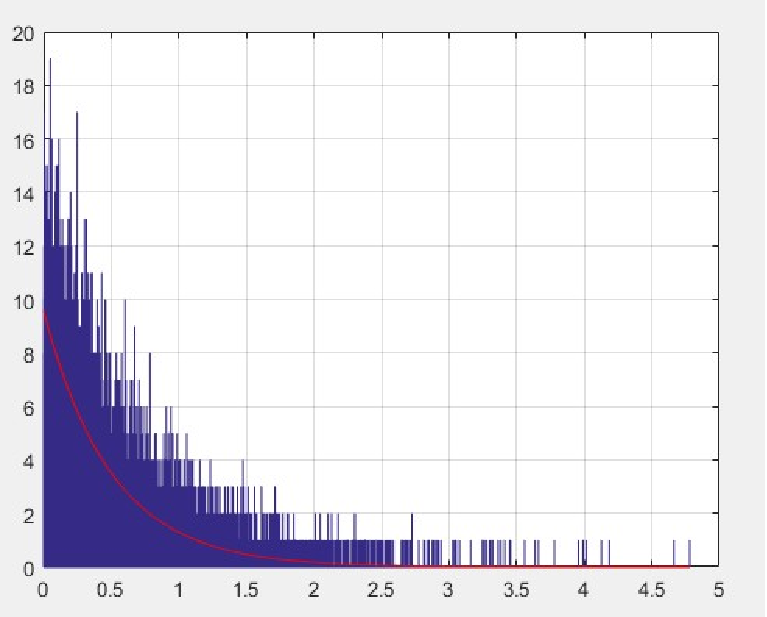
\includegraphics[width=0.4\linewidth]{img/kich_bur/image1}
	\caption{Гистограмма случайной величины $ R $, $r_i \sim Exp(\lambda),i=(1,n) $ распределенная по экспоненциальному закону, количество элементов последовательности $ n=10000, \lambda=0,5 $}
	\label{fig:img1}
\end{figure}

$Exp(\lambda),i=1,n$
распределенная по экспоненциальному закону, количество элементов последовательности
$n=10000$, $\lambda=0,5$ 


Мат.ожидание случайной величины $ R $ распределенной по экспоненциальному
закону = $ 0.5009  $

Дисперсия случайной величины $ R $ распределенной по экспоненциальному
закону = $ 0.2532 $ 

Получим величину $R^{'}$ как $r_{i}^{'}=r_{i}-t_{1}$ и оставим
только те значения, которые $r^{'}\geq0$ . Пусть количество этих
новых значений равно $n^{'}$ . Пусть $t_{1}=0.7$

\begin{figure}[h]
	\centering
	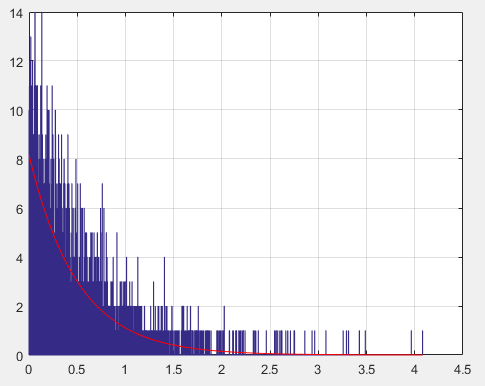
\includegraphics[width=0.4\linewidth]{img/kich_bur/image2}
	\caption{Гистограмма случайной величины $ R^{'} $}
	\label{fig:img2}
\end{figure}

\begin{figure}[h]
	\centering
	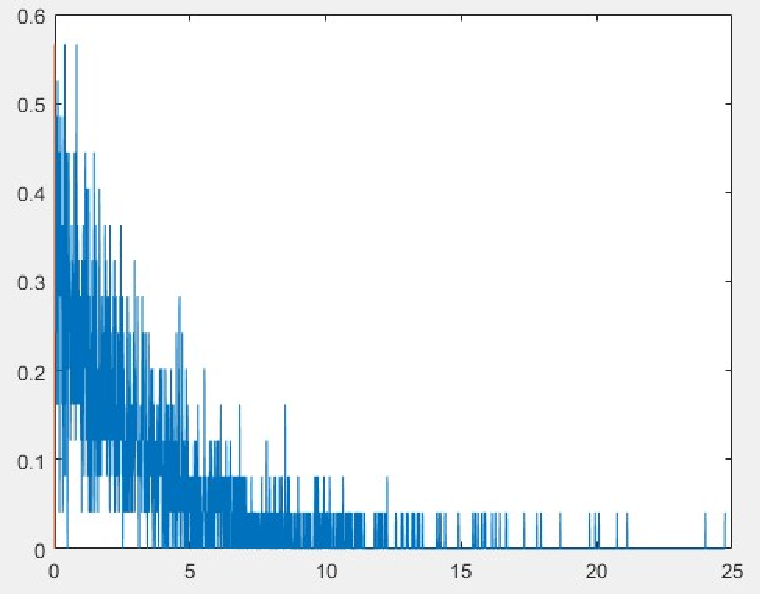
\includegraphics[width=0.4\linewidth]{img/kich_bur/image3}
	\caption{График плотности вероятности случайной величины $ R^{'} $}
	\label{fig:img3}
\end{figure}

$M[R^{'}]= 0.5024$

Количество элементов на второй итерации $n^{'}=2473$

Дисперсия на второй итерации $D[R^{'}] = 0.2587 $

Получим величину $R^{''}$ как $r_{i}^{''}{}^ {}=r_{i}^{'}-t_{2}$
и оставим только те значения, которые $r^{''}\geq0$. Пусть количество
этих новых значений равно $n^{''}$. Пусть $t_{2}=0.3.$ 
\begin{figure}[h]
	\centering\
	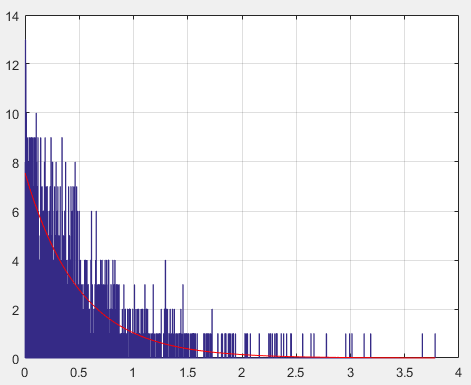
\includegraphics[width=0.4\linewidth]{img/kich_bur/image4}
	\caption{Гистограмма случайной величины $R^{''}$ }
	\label{fig:img4}
\end{figure}

Мат.ожидание после шага 2: $M[R^{''}]= 0.4947 $

Количество элементов на второй итерации: $n^{''}= 1381 $

Дисперсия на третьей итерации: $D[R^{''}]= 0.2638 $

Для сравнения проведем аналогичный опыт, сгенерировав последовательность
по закону Пуассона. Сгенерирована случайная величина $ RN $, $rn_{i}\sim
P(\lambda),i=1,n$ распределенная по закону Пуассона, количество элементов
последовательности $n=10000$, $\lambda=4$.
 
\begin{figure}[h]
	\centering
	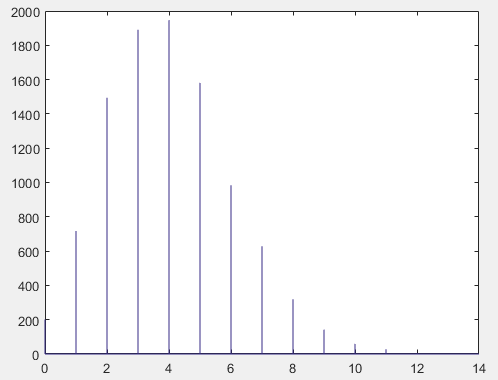
\includegraphics[width=0.4\linewidth]{img/kich_bur/image5} 
	\caption{Гистограмма случайной величины распределенной по закону Пуассона}
	\label{fig:img5}
\end{figure}

Сравним результаты. Для экспоненциального распределения: 

$M[R]= 4.0269$ 

$D[R]= 15.8816$ 

Мат.ожидание для распределения по закону Пуассона: 

$M[RN]= 4.0212$ 

Дисперсия для распределения по закону Пуассона: 

$D[RN]= 4.1518$ 

Получим величину $R^{'}$ и $RN^{'}$ как $r_{i}^{'}=r_{i}-t_{1}$
и $rn_{i}^{'}=rn_{i}-t_{1}$ оставим только те значения, которые
${r^{'}}$ и ${rn^{'}\geq0}$. Пусть количество этих новых
значений равно $n^{'}$ и $nr^{'}$ . Пусть $t_{1}=0.7.$ 

$M[R']= 4.0471$ 

количество элементов на второй итерации: 

$n'= 8366$ 

дисперсия на второй итерации: 

$D[R^{'}]=15.8007$

$M[RN']= 3.4033$ 

$D[RN']= 3.8984$ 

Для сравнения проведем аналогичный опыт, сгенерировав последовательность
по равномерному закону. Сгенерирована случайная величина RR, $rr_{i}\sim P(n),i=1,n$
распределенная по равномерному закону, количество элементов последовательности
$ n=10000  $
\begin{figure}[h]
	\centering
	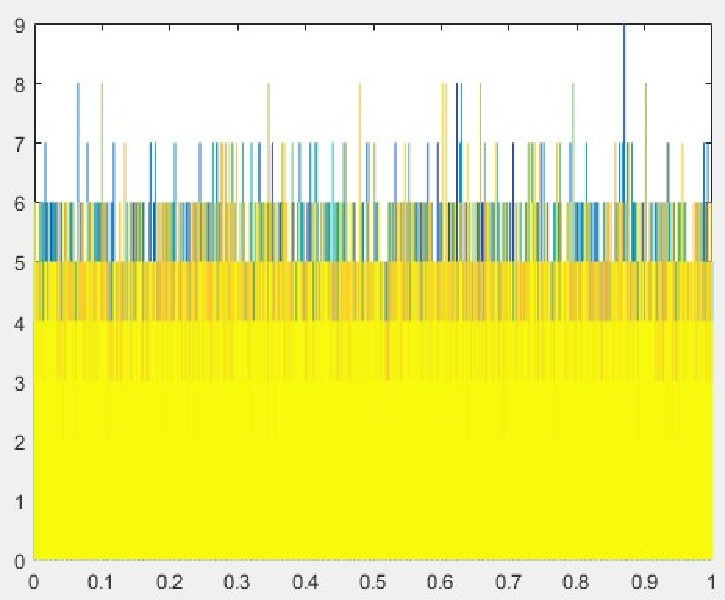
\includegraphics[width=0.4\linewidth]{img/kich_bur/image6} 
	\caption{Гистограмма случайной величины $RR$ }
	\label{fig:img6}
\end{figure}

Мат.ожидание для распределения по равномерному закону $M[RR]=0.4906$ 

Дисперсия для распределения по равномерному закону $D[RR]=0.0834$

Мат.ожидание после шага 1 по равномерному закону $M[RR']=
0.1472 $

Количество элементов на второй итерации по равномерному закону $n'=
295 $

Дисперсия на второй итерации по равномерному закону \[ D[RR^{'}]=0.0075 \]
\begin{figure}[h]
	\centering
	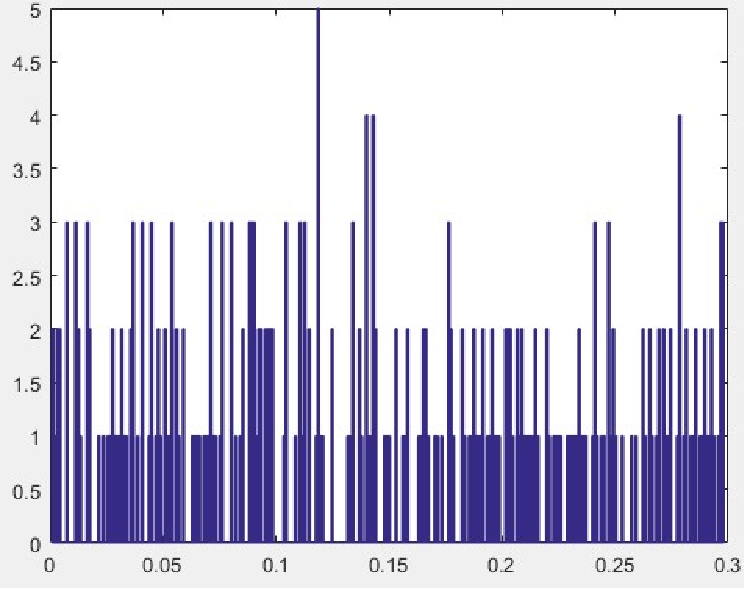
\includegraphics[width=0.4\linewidth]{img/kich_bur/image7} 
	\caption{Гистограмма случайной величины $RR^{'}$}
	\label{fig:img7}
\end{figure}

Сгенерируем две последовательности распределенные по
экспотенциалному закону по n случайных величин:  $R,$
$rd_{i}\sim Exp(\lambda)+sim Exp(\lambda),i=1,n$.
Вычисли мат.ожидание и дисперсию. Затем получим случайную величину $Rd^{'}$ как
$rd_{i}^{'}=rd_{i}-t_{1}$ и оставим только те значения, которые $rd^{'}\geq0$ .
Пусть количество этих новых значений равно $nd^{'}$ . Пусть $t_{1}=0.7$

Мат.ожидание суммы двух случайных величин $ Rd $ распределенных по
экспоненциальному закону = $ 8.3967  $

Дисперсия суммы двух случайных величин $ Rd $ распределенных по
экспоненциальному закону = $ 34.2300 $ 
\[ M[Rd^{'}]= 7.7769; D[Rd^{'}]= = 33.9038; nd^{'}= 990 \]
 

\subsection{Выводы}

\[ M[R]= 0.5009; D[R]= 0.2532  \]


\[ M[R^{'}]= 0.5024; D[R^{'}]= = 0.2587 \]


\[ M[R^{''}]= 0.4947; D[R^{''}]= 0.2638 \]


\[ M[RN]= 4.0212; D[RN]=4.1518 \]


\[ M[RN']= 3.4033; D[RN']= 3.8984 \]


\[ M[RR]= 0.4906; D[RR]= 0.0834 \]


\[ M[RR']= 0.1472; D[RR']= 0.0075 \]

\[ M[Rd]= 8.3967; D[Rd]= 34.2300 \]

\[ M[Rd^{'}]= 7.7769; D[Rd^{'}]= 33.9038 \]

Вычислив $M[R^{'}]$ и $D[R^{'}]$ получим, что:
\[ M[R]=M[R^{'}]\]
\[D[R]=D[R^{'}] \]

Таким образом, для случайной величины распределенной по экспоненциальному
закону, эффект отсутствия памяти работает. Утверждение справедливо
только в том случае, если случайная величина распределена по экспоненциальному
закону, что соответствует теории и результатам моделирования. Сумма двух
случайных величин, распределенных по экспоненциальному закону, данным эффектом не
обладает.

Код программы на Matlab [\ref{code:Kishkun.code1}]:
%\label{code:code1}
\lstinputlisting[language=Matlab, frame=single,
label=code:Kishkun.code1, caption=Программа моделирования]{src/1.m}
\newpage
 	% !TeX spellcheck = ru_RU
% !TeX encoding = UTF-8
\section{Sigfox.Кишкун. Задание 3}
\subsection{Назначение системы}
Компания \textbf{Sigfox} (Франция) занимается разработкой и внедрением технологии сверх узкополосной (\textbf{UNB} — Ultra Narrow Band) беспроводной связи для передачи данных в субгигагерцовом нелицензируемом диапазоне 868.8 MГц. Сеть компаний развернута в Европе: Франция, Италия, Великобритания, Ирландия, Испания, Португалия, Люксембург, Нидерланды, Бельгия, Дания. 

Основная разработка Sigfox — энергоэкономные беспроводные сети, которые станут основой интернета вещей. Благодаря этим сетям между собой смогут обмениваться данными «умные» часы, телевизоры, микроволновые печи, стиральные машины и другие устройства. Эта технология изначально предназначена для связи на низких скоростях передачи данных. SigFox в настоящее время использует самый популярный европейский \textbf{ISM} диапазон на 868 МГц (как определено стандартом ETSI и СЕРТ), а также 902 МГц в США (как определено FCC), в зависимости от конкретных региональных правил. Система развернута с использованием возможностей современных сотовых сетей.
\subsection{Структура системы}
Устройство может отправить до 140 сообщений в день, и каждое сообщение может содержать до 12 байт полезных данных. 12 байт покрывает потребности устройств, которые передают данные, такие как местоположение устройства, индекс потребления энергии, сигнал тревоги или любой другой тип основной сенсорной информации. 
Также можно передавать до 4 сообщений из 8 байт полезных данных на каждое устройство в сутки. Для того, чтобы получать сообщения, устройство должно запросить данные с сервера, это должно быть запрограммировано на конкретные события или на определенное время, что позволяет экономить энергию, находясь большую часть времени в спящем режиме. 8 байт, отправленные на устройство, позволяют при необходимости отправить данные конфигурации, можно оптимизировать срок службы аккумулятора. Этого достаточно, если нет необходимости в полноценной двусторонней связи. На данный момент система Sigfox реализована с односторонней связью: данные с датчиков агрегируются и передаются на сервера компании Sigfox(\ref{fig:img11}). 
\begin{figure}[H]
	\centering
	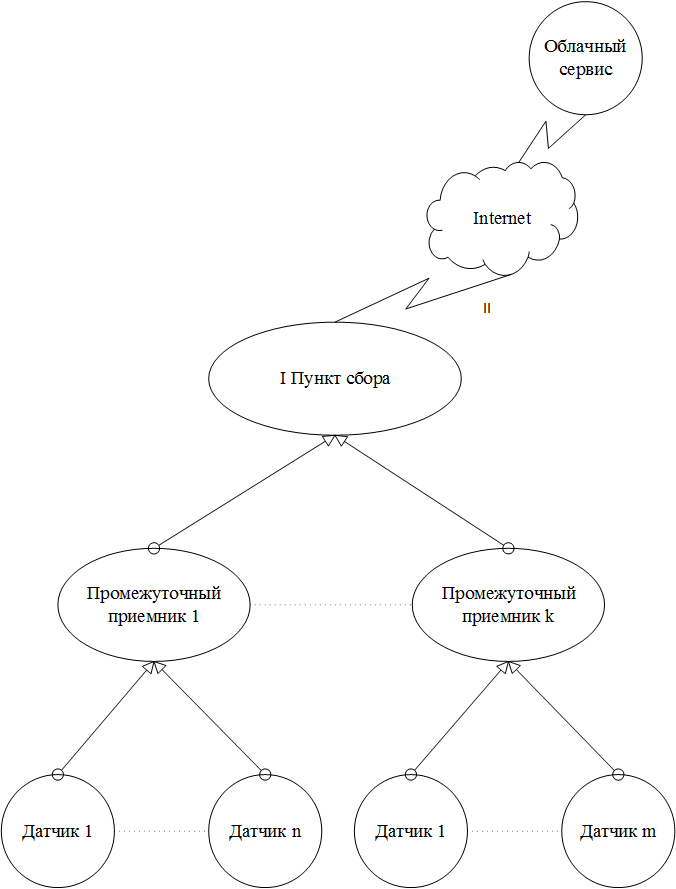
\includegraphics[width=0.5\textwidth]{img/kich_bur/11.png}
	\caption{Стурктура системы Sigfox}
	\label{fig:img11}
\end{figure}
\subsection{Разбиение системы на уровни}
Sigfox — исторически первая крупная компания на рынке интернета вещей — выбрала для себя довольно закрытую модель. На рисунке \ref{fig:img12} представлено разбиение системы на уровни. У Sigfox необходимо купить базовые станции и заключить с ним договор на разворачивание сети, к которой будет предоставляться платный доступ сторонним абонентам. Базовые станции передают данные на сервера Sigfox, то есть канал связи --- не физический, но логический и ПО верхнего уровня также принадлежат Sigfox. Sigfox не стал узурпировать рынок чипов и конечных устройств --- он договорился с Texas Instruments, SiLabs и другими производителями о поддержке своей сети, что позволяет заказать какое-то нестандартное Sigfox-устройство. К сожалению, проблему может составить его подключение к сети: если в Европе Sigfox успел развернуться, то сейчас, с появлением LoRa, его экспансия фактически остановилась.
Сотовые сети LPWAN --- сети масштаба городов --- это сети с множеством базовых
станций (например, на покрытие Москвы надо порядка 200 штук), как правило, обслуживаемые оператором сети, предоставляющим за деньги доступ к ней владельцам конечных устройств. Sigfox устанавливает жесткую тарифную сетку. 
\begin{figure}[H]
	\centering
	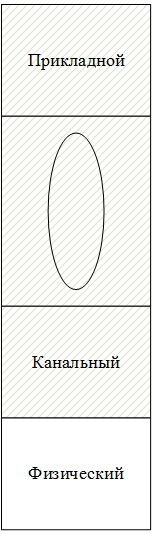
\includegraphics[width=0.2\textwidth]{img/kich_bur/12.png}
	\caption{Разбиение системы Sigfox на уровни}
	\label{fig:img12}
\end{figure}
Таким образом, все уровни закрыты, за исключением физического, что позволяет
сделать гибкую сетку маломощных устройств. 
\subsection{Особенности построения уровней}
Sigfox не поддерживает топологию «звезда». Ни в Sigfox, ни в «Стриже», ни вообще в мире узкополосных UNB-систем сети такой топологии технически невозможны: из-за специфики UNB-систем абонентское устройство в общем случае не может принимать данные в произвольные моменты времени от других абонентских устройств, а значит, не может выступать в качестве ретранслятора.
Все решения распадаются на две группы: широкополосные UWB (Ultra Wide Band, к ним из перечисленного относится только LoRa) и узкополосные UNB (Ultra Narrow Band, в нашем случае это Sigfox и «Стриж»). Из этого проистекает ряд отличий.
UWB: один канал занимает полосу в эфире с шириной 125 или 250 кГц
UNB: один канал занимает полосу в эфире с шириной 100 Гц

В России в диапазоне, условно именуемом «\textbf{868 МГц}», для
неспециализированных устройств официально доступны две полосы частот:
864,0-865,0 МГц с периодом активной работы не более одной десятой процента и
запретом на работу вблизи аэропортов и 868,7-869,2 МГц без таких ограничений. В общем случае мы имеем всего лишь 500 кГц доступной нам полосы частот. Каналов Sigfox при ширине 125 кГц в эту полосу умещаются сотни.

В UNB-системах один приёмник базовой станции в один момент времени может принимать только один канал.  Термин «частотное разделение» относится к способности приёмника выцепить этот канал из общего эфира так, чтобы на него не накладывалась передача в соседних каналах — и если мы в данную секунду принимаем что-то по каналу N, то по каналам N+1 и N-1 мы принять в это же время ничего не можем. В UWB-системах используется не только частотное и временное, но и кодовое разделение каналов.  

Из-за допплеровского эффекта Sigfox теряет стабильность работы уже на скорости движения конечного устройства в районе 5-10 км/ч. 

UNB-системы работают на фиксированной низкой скорости. У Sigfox скорость передачи данных 100 бит/с, у «Стрижа» — 50 бит/с.

Дальность связи во всех подобных технологиях очень сильно зависит от условий на местности: в целом можно считать, что все перечисленные технологии обеспечивают дальность 1-3 км в городской застройке и 15-20 км на открытой местности. Дальность может быть увеличена за счёт выгодного расположения антенн: например, слова «в городской застройке» могут означать как абонентские устройства, расположенные в глубине зданий и оснащённые компактными печатными антеннами, так и управлемые уличные фонари с обычными штыревыми антеннами, стоящими на открытом воздухе и минимум в пяти метрах от земли.
Энергопотребление сверхнизкое, по оценкам до 20 лет работы сенсора от 2-х батарей АА. 

\newpage
	% !TeX spellcheck = ru_RU
% !TeX encoding = UTF-8
\subsection{АБГШ}
\label{sec:awgn}

Аддитивный Белый Гауссовский Шум (АБГШ) является видом мешающего воздействия в канале связи или других процессах. Определяется данный вид шума как гауссовский случайный процесс $n(t )$ с нулевым средним и спектральной плотностью мощности $S_n( f ) = N_0 / 2$. АБГШ является наиболее распространённым видом шума, используемым для расчёта и моделирования систем связи. Термин «аддитивный» означает, что данный вид шума суммируется с исходным сигналом и статистически не зависим от сигнала.

Дисперсия АБГШ может быть вычислена как $\sigma^2 = \int_{-\infty}^{\infty}S_n(f)df$. Так как АБГШ существует во всей полосе частот $-\infty < f < \infty$, то $\sigma^2 = \infty$. В реальности такого не может существовать, т.к. бесконечно большой мощности не может быть. Шум не может существовать без сигнала, таким образом, ширина полосы частот шума зависит от ширины полосы частот исходного сигнала. 
	% !TeX spellcheck = ru_RU
% !TeX encoding = UTF-8
\section{Теоретическая вероятность в двоичном канале с аддитивным белым гуассовским шумом}

Рассмотрим систему передачи двоичных сигналов $0$ и $1$. Вероятность ошибки в такой системе определяется по следующей формуле:

\begin{equation}
	P_e = \sum_{i=0}^{1}P_e(i)P_i = P_e(0)P_0 + P_e(1)P_1,
\end{equation}

где $P_e(i)$ -- условная вероятность ошибки при передаче $i$-го сигнала, $P_i$ -- вероятность передачи $i$-го сигнала. Рассмотрим простую систему с одинаковыми вероятностями передачи сигналов. Таким образом, можно рассчитать вероятность ошибки для одного символа, эта же вероятность будет являться вероятностью ошибки для всей системы. Вероятность ошибки будем рассчитывать по максимальному правдоподобию:
\begin{equation}
	\label{form:pe_1}
	P_e(0) = Pr[d^2(r,s_0) > d^2(r,s_1) \mid 0] = Pr[ || r - s_0||^2 > ||r - s_1||^2 \mid 0] ,
\end{equation}

где $r$ -- принятый сигнал, $s_i$ -- переданный $i$-ый сигнал. При этом нужно учесть, что $r = s_i + n$, где $n$ -- АБГШ, который описан в разделе \ref{sec:awgn}. Тогда формула (\ref{form:pe_1}) приобретает вид:
\begin{equation}
	P_e(0) = Pr[||n||^2 > ||s_0 - s_1 + n||^2] = Pr[||n||^2 - ||s_0 - s_1 + n||^2 > 0].
\end{equation}
Выражение $||n||^2 - ||s_0 - s_1 + n||^2$ при раскрытии скобок преобразуется в 
\begin{equation}
\begin{split}
	||n||^2 - ||s_0 - s_1 + n||^2 = ||n||^2 - ||s_0 - s_1||^2 - 2\sum_{j=1}^{D}(s_{0j} - s_{1j}) n_j\\ - ||n||^2 = 
	 - ||s_0 - s_1||^2 - 2\sum_{j=1}^{D}(s_{0j} - s_{1j}) n_j.
\end{split}
\end{equation}
Произведем замену переменных $\Delta^2 =-2||s_0 - s_1||^2$ и $\epsilon =  -2\sum_{j=1}^{D}(s_{0j} - s_{1j}) n_j$, тогда 
\begin{equation}
	P_e(0) = Pr[\epsilon > \Delta^2].
\end{equation}
Стоит отметить, что $\epsilon$ является случайной гуассовской величиной, т.к. является линейной комбинацией разности сигналов и АБГШ. Принимая в расчет, что математическое ожидание АБГШ равно $0$, то $\bar{\epsilon} = 0$, а дисперсия $D[\epsilon] = 2N_0\Delta^2$.

Для дальнейших расчетов необходимо ввести Q-функцию, которая позволяет найти вероятность превышения некоторого порога $A$ гауссовской случайной величиной $x$ с параметрами $(m,\sigma^2)$:

\begin{equation}
	Pr[x > A] = Q(\frac{A - m}{\sigma}).
\end{equation}

Q-функция определяется следующей формулой:

\begin{equation}
	Q(x) = \int_{x}^{\infty}{\frac{1}{\sqrt{2\pi}}}e^{-z^2 / 2}dz
\end{equation} 

С учетом вышесказанного:
\begin{equation}
	P_e(0) = Q(\frac{\Delta^2}{\sqrt{\Delta^22N_0}}) = Q(\frac{\Delta}{\sqrt{2N_0}}).
\end{equation}

Так как $P_e(0)$ = $P_e(1)$, то
\begin{equation}
	P_e = Q(\frac{\Delta}{\sqrt{2N_0}}).
\end{equation}

Таким образом, вероятность ошибки дыоичных сигналов в канале с АБГШ зависит от величины евклидова расстояния между сигналами и интенсивности шума. При этом стоит учесть, что вид сигналов значения не имеет.
	% !TeX spellcheck = ru_RU
% !TeX encoding = UTF-8
\subsection{Почему зону покрытия абонентской станции изображают шестиугольником}

%шестиугольником можно покрыть пространство без дыр, так же, как и квадратом или треугольником
%шестиугольник ближе к кругу, ежели квадрат или треугольник
%диаграммы воронова


На заре развития беспроводной связи перед исследователями и инженерами-связистами встала задача, как изображать границы принимаемого сигнала Абонентскими Станциями (АС). По своей природе АС имеют круговую диаграмму направленности. Но если изображать границы сигнала кругами, то карта АС становится перегруженной. Из геометрии известно, что существует три типа многоугольников, которыми можно заполнить пространство: треугольники, квадраты и шестиугольники. Из этих трех фигур шестиугольник ближе всего к кругу, которым описывается граница области покрытия АС. 

При этом стоит отметить, что шестиугольники удобны только в случае АС с одинаковой мощностью и зоной покрытия, расположенные по сетке с одинаковым шагом. Когда на области существуют разные виды АС, которые удалены друг от друга на разное расстояние, используют диаграммы Вороного. 

\subsubsection{Диаграмы Вороного}

Диаграммы Вороного используются во многих областях жизнедеятельности человека, в том числе телекоммуникациях. Для начала введем понятия нужных для понимания геометрических объектов:

\begin{itemize}
	\item Простой многоугольник -- это многоугольник без самопересечений. Мы будем рассматривать только простые многоугольники.
	\item Невыпуклый многоугольник -- это многоугольник, в котором есть такие две вершины, что через них проводится прямая, пересекающая данный многоугольник где-либо ещё, кроме ребра, соединяющего эти вершины (рисунок \ref{fig:mnogoug}), 
	\item Выпуклый многоугольник -- это многоугольник, у которого продолжения сторон не пересекают других его сторон рисунок \ref{fig:mnogoug}).
\end{itemize}

\begin{figure}[h]
	\centering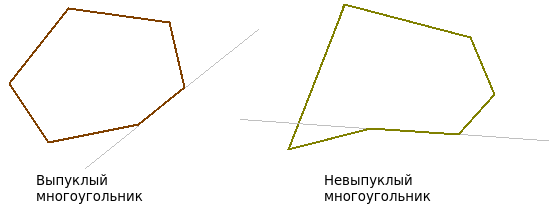
\includegraphics[width=0.7\linewidth]{mnogoug}
	\caption{Примеры выпуклого и невыпуклого многоугольников}
	\label{fig:mnogoug}
\end{figure}

Именно из выпуклых многоугольников и будет состоять диаграмма, так как они являются ничем иным, как пересечением полуплоскостей, которые являются выпуклыми фигурами.

Диаграмма состоит из локусов -- областей, в которых присутствуют все точки, которые находятся ближе к данной точке, чем ко всем остальным. В диаграмме Вороного локусы являются выпуклыми многоугольниками.

По определению локус строится следующим образом: пусть дано множество из $n$ точек, для которого мы строим диаграмму. Возьмём конкретную точку $p$, для которой строим локус, и ещё одну точку из данного нам множества $q$ не равную $p$. Проведём отрезок, соединяющий эти две точки, и проведём прямую, которая будет являться серединным перпендикуляром данного отрезка. Эта прямая делит плоскость на две полуплоскости. В одной лежит точка $p$, в другой лежит точка $q$. В данном случае локусами этих двух точек являются полученные полуплоскости. То есть для того, чтобы построить локус точки $p$, нужно получить пересечение всех таких полуплоскостей. То есть на месте $q$ должны быть все точки данного множества, кроме $p$.

\begin{figure}[h]
	\centering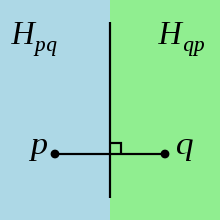
\includegraphics[width=0.3\linewidth]{polupl}
	\caption{Пример полуплоскостей}
	\label{fig:polupl}
\end{figure}

Точку, для которой строится локус, называют сайтом (site). На рисунке \ref{fig:sites} локусы помечены разными цветами.

\begin{figure}[h]
	\centering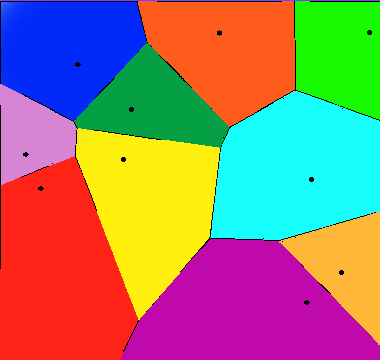
\includegraphics[width=0.4\linewidth]{sites}
	\caption{Сайты в диаграмме Вороного}
	\label{fig:sites}
\end{figure}

Алгоритмы построения диаграммы строят локусы для всех точек из заданного набора. Локусы в данной задаче также называют многоугольниками Вороного или ячейками Вороного. 

Наконец, сформулируем определение диаграммы Вороного $n$ точек на плоскости -- это разбиение плоскости, состоящее из $n$ локусов. 

\subsubsection{Алгоритм построения диаграммы Вороного}

Основная идея алгоритма в том, чтобы пересекать не полуплоскости, а именно серединные перпендикуляры отрезков, так как это проще, соединяющих данную точку со всеми другими точками. То есть, следуя определению ячейки Вороного, мы будем строить локус для точки $p$ следующим образом:

\begin{enumerate}
	\item Получаем $n-1$ прямую (серединные перпендикуляры), так как мы провели серединные перпендикуляры всех отрезков, соединяющих данную точку $p$ с остальными;
	\item Пересекаем попарно все прямые, получаем $O(n^2)$ точек пересечения (потому что каждая прямая может пересечь все другие, в «худшем случае»);
	\item Проверяем все эти $O(n^2)$ точек на принадлежность каждой из $n-1$ полуплоскостей, то есть получаем уже асимптотику $O(n^3)$. Соответственно те точки, которые принадлежат всем полуплоскостям, и будут вершинами ячейки Вороного точки $p$;
\end{enumerate}

Проделываем первые три шага для всех $n$ точек, получаем итоговую асимптотику $O(n^4)$.

    % !TeX spellcheck = ru_RU
% !TeX encoding = UTF-8
\section{Нагрузка на сеть в Эрлангах}

Эрланг (обозначение Эрл) — безразмерная единица интенсивности нагрузки (чаще всего телефонной
нагрузки) или единица нагрузки, используемая для выражения величины нагрузки, требуемой для 
поддержания занятости одного устройства в течение определённого периода времени.

1 эрланг (1 Эрл) --- соответствует непрерывному использованию одного голосового канала в течение
1 часа. То есть если абонент проговорил с другим абонентом в течение одного часа, то на 
телекоммуникационном оборудовании была создана нагрузка в один эрланг.

Оценка телекоммуникационного трафика в эрлангах позволяет вычислить количество необходимых каналов
в конкретной зоне (области, базовой станции). Эрланг используется операторами связи для учёта 
пропускной способности при транзите трафика, так как телефонная нагрузка --- это случайная величина,
которая определяется количеством поступивших вызовов за единицу времени и временем обслуживания
абонента. Интенсивность нагрузки является произведением матожидания числа вызовов за единицу времени
на среднее время обслуживания вызова; эта интенсивность и измеряется в эрлангах. Важно отметить, что
введение рассматриваемой единицы, существенно, упростило расчёт нагрузки на сеть.

Единица названа в честь датского математика и инженера Агнера Крарупа Эрланга, который предложил
использовать математический анализ для учёта телефонной нагрузки. Агнер Эрланг проводил анализ
работы местной телефонной станции одной деревни, жители которой пытались установить соединение с
абонентами других населённых пунктов. В 1909 году им была опубликована работа «Теория вероятностей
и телефонные разговоры», в результате чего метод и стал популярным.
    % !TeX spellcheck = ru_RU
% !TeX encoding = UTF-8
\section{Защитный интервал}
В английской литературе защитный интервал --- Guard Interval.
Важно сразу отметить, существуют различные техники для борьбы с помехами при передаче по радио 
каналу. В данном разделе будет рассмотрен <<Защитный интервал>>, как средство для борьбы со взаимной
интерференцией сигнала рисунок~\ref{fig:kov_interf}, возникающей в следствие наличия замираний в канале.

Если путь от передатчика к приемнику имеет отражения или 
препятствия, либо и то и другое, мы можем получить эффект замирания. В этом случае, сигнал достигает
приемника разными путями, каждый из которых --- копия оригинала. Каждый из этих лучей имеет
немного разную задержку и немного разное усиление. Временные задержки выливаются в
фазовые сдвиги, которые накладываются на компоненту основного сигнала (если таковой
имеется), вызывая ухудшение сигнала.

\begin{figure}[H]
    \centering
    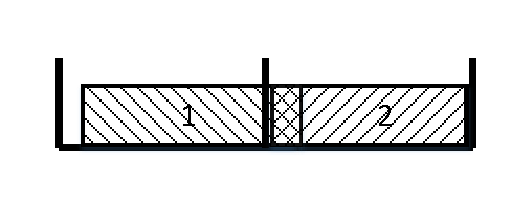
\includegraphics[width=0.5\textwidth]{img/kov_interf}
    \caption{Интерференция двух сообщений}
    \label{fig:kov_interf}
\end{figure}

Защитным интервалом называют дополнение к сообщению, передаваемому по каналу, куда вставляется
циклический префикс (ЦП), где ЦП --- копия конца сообщения~\ref{fig:kov_CP} .

\begin{figure}[H]
    \centering
    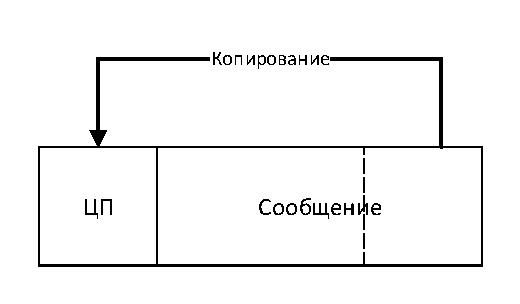
\includegraphics[width=0.5\textwidth]{img/kov_CP}
    \caption{Циклический префикс}
    \label{fig:kov_CP}
\end{figure}

Таким образом, если часть сообщения будет нарушена, как на рисунке~\ref{fig:kov_interf}, полезная 
информация не будет потеряна, так как дубликат хранится в ЦП, что позволяет полностью восстановить
сообщение на приёмной стороне, даже при наличии взаимной интерференции между сообщениями.
    \subsection{Защитный интервал в сетях LTE}
Рассмотрим систему, изображенную на рисунке~\ref{fig:vol_mobile_cell}.
\begin{figure}[H]
    \centering
    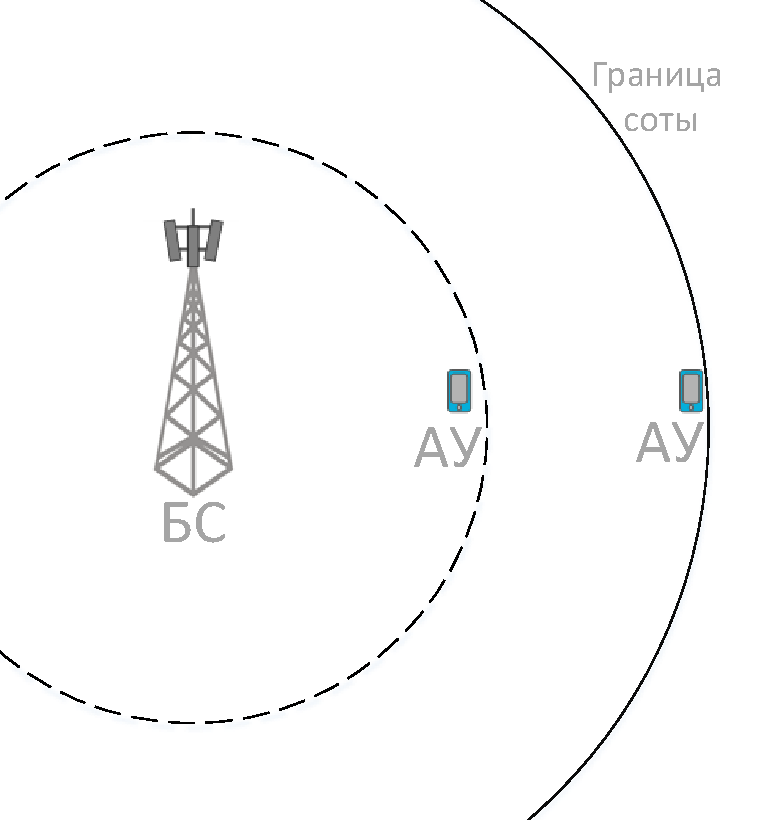
\includegraphics[width=0.5\textwidth]{img/vol_mobile_cell}
    \caption{Мобильная сота с двумя абонентами}
    \label{fig:vol_mobile_cell}
\end{figure}

Данная система состоит из базовой станции (БС) и двух абонентских устройств (АУ), один из которых
расположен непосредственно у базовой станции, второй --- на границе соты. Ни АУ, ни БС не могут знать
точное время появления данных в пределах установленного окна, так как информация передается с
некоторой задержкой. Если задержка одного из передаваемых сообщений окажется слишком большой, то
данное сообщение выйдет за границы собственного окна. Это может привести к наложению одного сообщения
на другое --- к интерференции, в результате которой принятые сообщения будет невозможно корректно
обработать. Подобный случай приведен на рисунке~\ref{fig:vol_interf}
\begin{figure}[H]
    \centering
    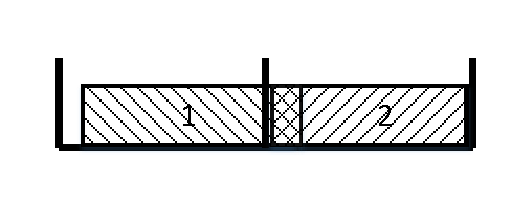
\includegraphics[width=0.5\textwidth]{img/vol_interf}
    \caption{Интерференция двух сообщений}
    \label{fig:vol_interf}
\end{figure}
Для устранения подобного эффекта вводится специальный параметр --- защитный интервал.
При использовании данного параметра время передачи сообщения сокращается. Освободившийся интервал
времени (защитный интервал) делится на две части: циклический префикс (ЦП) и защитное время (ЗВ).
ЦП является избыточной информацией и представляет собой повторение конца сообщения.
Он необходим для корректной обработки в тех случаях, когда сообщение вышло за границы
собственного окна. ЗВ необходим для того, чтобы снизить влияние задержки на передачу сообщений
абонентам, находящимся на больших расстояниях от базовой станции. Пример такого случая
приведен на рисунке~\ref{fig:vol_CP}. 
\begin{figure}[H]
    \centering
    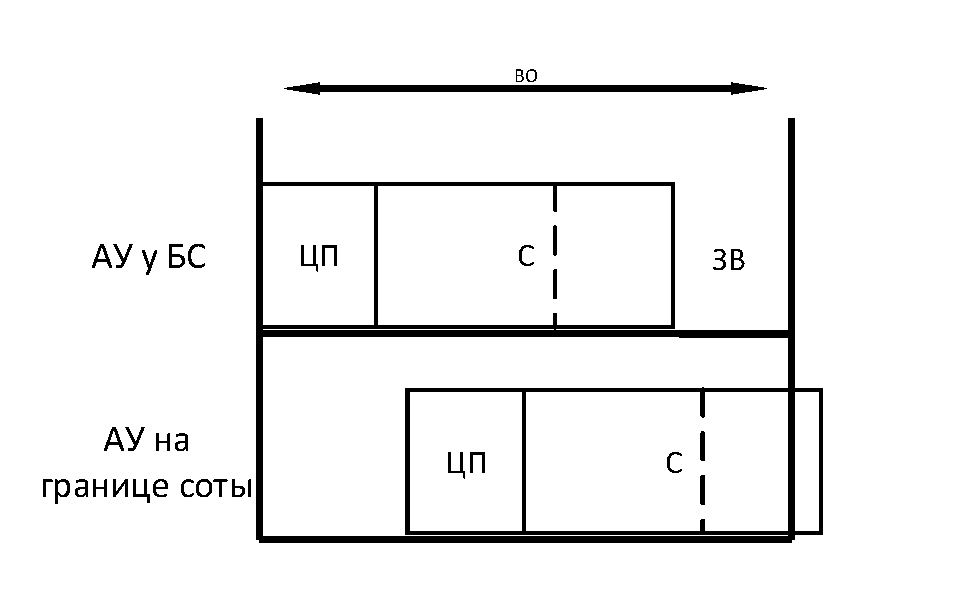
\includegraphics[width=0.75\textwidth]{img/vol_CP}
    \caption{Использование циклического префикса}
    \label{fig:vol_CP}
\end{figure}

Ошибки синхронизации, различные задержки при передаче сообщений приводят к интерференции.
Использование ЦП и ЗВ позволяет сократить возможность возникновения подобного явления.

Выбор размера ЦП и ЗВ во многом зависит от характера местности и размера соты. Для определения
влияния размера соты на значение ЦП рассмотрим рисунок~\ref{fig:vol_calc_CP}.
\begin{figure}[H]
    \centering
    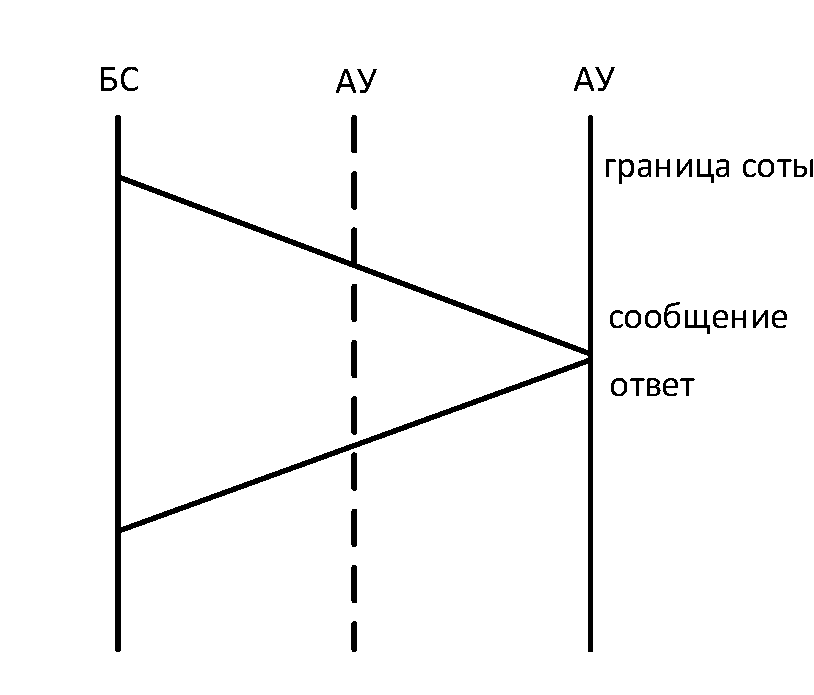
\includegraphics[width=0.5\textwidth]{img/vol_calc_CP}
    \caption{Передача сообщения от БС к АУ на границе соты}
    \label{fig:vol_calc_CP}
\end{figure}

Известно, что радиосигнал распространяется со скоростью примерно равной скорости света \(c = 3 \cdot
10^{8}\) м/с. Таким образом, время распространения сигнала от БС до дальнего АУ равно
\(T = \dfrac{Cell Size}{c}\). Но для завершения передачи БС должна получить ответ от АУ.
Время распространения ответа равно времени распространения сообщения \(T = \dfrac{2 \cdot Cell
Size}{c}\). Таким образом, через время, равное \(Т\), сообщение поступит на АУ, а спустя небольшую
задержку поступят переотраженные сигналы \((d)\).
Отсюда можно сделать вывод, что размер защитного интервала должен быть равен времени распространения
сигнала. В итоге размер циклического префикса равен \[T_{CP} = T = \dfrac{2 \cdot Cell Size}{c} + d\].


    % !TeX spellcheck = ru_RU
% !TeX encoding = UTF-8
\section{Передача радио сигнала <<за горизонт>>. Эффект Кабанова}
На сегодняшний день частотный ресурс распределяется Государственной комиссией по радиочастотам.
Государственная комиссия по радиочастотам (ГКРЧ) — межведомственный координационный орган, действующий при Министерстве связи и массовых коммуникаций Российской Федерации. ГКРЧ обладает всей полнотой полномочий в области регулирования радиочастотного спектра и отвечает за формирование государственной политики в области его распределения и использования. Помимо этого, комиссия готовит позицию Администрации связи Российской Федерации на все форумы Международного союза электросвязи для защиты интересов страны на международном уровне и международно-правовой защиты орбитально-частотного ресурса Российской Федерации. В рамках Комиссии проводятся исследования, по совершенствованию механизмов регулирования использования радиочастотного спектра, обеспечению электромагнитной совместимости радиоэлектронных средств, решению проблем внедрения на сетях связи России новых радиотехнологий.

Долгое время после того, как было изобретено рядио, считалось, что для целей связи наиболее приемлемы
длинные волны, так как они позволяют устанавливать связь на больших расстояниях, чем короткие.
Казалось, что короткие волны, в отличие от длинных, не в состоянии распространяться на значительные
расстояния за горизонт. Теперь весь мир. пронизывает радиосвязь на коротких волнах, хотя до 1947 г.
никто не мог представить себе, чтобы радиосигнал, посланный на коротких волнах, можно было принять
в том же месте, откуда он послан.

Профессор, доктор технических наук Н. И. Кабанов (Новосибирский электротехнический институт) открыл
ранее неизвестное явление дальнего коротковолнового рассеяния радиоволн отдельными элементами
поверхности Земли. Радиоволны, излучаемые радиопередающим устройством под некоторым углом к горизонту,
отражаются ионосферой и идут обратно, к Земле. Часть их энергии рассеивается неоднородностями земной
поверхности и распространяется в разные стороны. Рассеянные радиоволны вновь отражаются от ионосферы
и возвращаются на Землю, причем какая-то их доля попадает и в то место, где находится радиопередающее устройство.

В 1950 г. Государственная комиссия под председательством академика А. И. Берга рассмотрела полученные
Н. И. Кабановым данные и дала следующее заключение: <<Настоящей работой впервые экспериментально установлено
существование регулярных рассеянных отражений от Земли на коротких волнах, что имеет принципиальное
значение для исследований условий распространения коротких волн, в частности применительно к эксплуатации
магистральных линий и средств дальней радионавигации>>.

Оригинальные эксперименты, поставленные Н. И. Кабановым, позволили обнаружить, что рассеяние радиоволн
гористыми участками Земли происходит более интенсивно, чем морями, подтвердили, что по границам дальности
отражений можно судить о состоянии ионосферы.

Использование эффекта Кабанова для исследования ионосферы (метод возвратно-наклонного зондирования)
дает возможность определять условия распространения радиоволн в радиусе до 9-12 тыс. км, т. е.
почти над четвертью поверхности земного шара. Метод возвратно-наклонного зондирования позволяет
значительно повысить надежность радиосвязи. Он особенно ценен тем, что используется в весьма загруженном
диапазоне коротких волн, обеспечивающих дальнюю радиосвязь. В нашей стране этот метод был разработан
и вошел в практику на два года раньше, чем за границей.

Эффект Кабанова находит применение также в ионосферной радиолокации и в других областях радиосвязи.
На основе эффекта Н. И. Кабанов и С. Г. Евскжов разработали способ радиолокационного загоризонтного
обзора поверхности Земли через ионизированные следы метеоров.

За рубежом эффект Кабанова получил всеобщее признание. Например, в Великобритании на ионосферной станции
в Слоу ведутся наблюдения за прохождением радиоволн с использованием коротковолнового рассеянного
отражения от Земли в радиусе до 6 тыс. км. В США разработаны сверхдальние загоризонтные радиолокаторы,
основанные на эффекте Кабанова.
    % !TeX encoding = UTF-8
% !TeX spellcheck = ru_RU
\section{Вычисление максимальной дальности}
\textbf{Кишкун. Задание 1}
В сетях первого поколения дальность передачи была обусловлена только
тем, что необходимой была прямая видимость между абонентом
и базовой станцией.
\subsection{Постановка задачи}
Как вычислить максимальное расстояние между абонентом и базовой станцией в зависимости от высоты, на которой они расположены? Геометрическое представление задачи изображено на рисунке \ref{fig:img8}.

\begin{figure}[H]
	\centering
	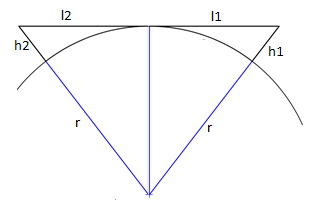
\includegraphics[width=0.5\textwidth]{img/kich_bur/image8.png}
	\caption{Геометрическое представление решаемой задачи}
	\label{fig:img8}
\end{figure}

$ h_1 $ --- высота антенны Базовой станции над поверхностью Земли 

$ h_2 $ --- высота антенны абонента над поверхностью Земли 

Земля --- идеальная сфера с радиусом $r = 6371$ км.

Максимальное расстояние между передатчиком и приемником будет тогда, когда прямая, соединяющая эти точки будет являться касательной к окружности. 

Предполагается, что частотный диапазон, мощность передатчика и чувствительность
приемника таковы, что если между передатчиком и приемником имеется
прямая видимость, то связь возможна вне зависимости от длины отрезка
между передатчиком и приемником. При относительно низких частотах
возможна передача за пределы прямой видимости. 

\subsection{Расчет физического расстояния}

Рассмотрим рисунок \ref{fig:img8}. По теореме Пифагора найдем длины $ l_1 $ и $ l_2 $: 

\[
(r+h_{1})^2=l_1^{2}+r_2
\]

\[
(r+h_{2})2=l_2^{2}+r_2
\]

\[
l1=\sqrt{h_{1}\left(h_{1}+2r\right)}
\]

\[
l2=\sqrt{h_{2}\left(h_{2}+2r\right)}
\]

Искомое расстояние: 

\[
L=\sqrt{h_{1}\left(h_{1}+2r\right)}+\sqrt{h_{2}\left(h_{2}+2r\right)}
\]

Расчет расстояния по поверхности: 

\[
\alpha_{1}=arctg(l_{1}/r)
\]

\[
\alpha_{2}=arctg(l_{2}/r)
\]

\[
C=(2*\pi*r*(\alpha1+\alpha2))/360
\]

\subsection{Доказательство оптимальности решения}
На рисунке \ref{fig:img9} показан случай, когда передатчик и приемник находятся дальше допустимого расстояния. Передаваемый сигнал будет гаситься землей.

\begin{figure}[H]
\centering{}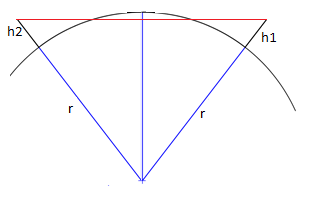
\includegraphics[width=3.27in,height=2.15in]{img/kich_bur/image9.png}
\caption{Превышение допустимого расстояния}
\label{fig:img9}
\end{figure}

Рассмотрим вариант, изображенный на рисунке \ref{fig:img10}. В этом случае передатчик и приемник находятся ближе допустимого расстояния. Сигнал будет проходить над поверхностью земли и расстояние между передатчиком и приемником не будет максимальным. 

\begin{figure}[H]
\centering{}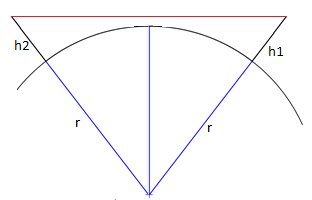
\includegraphics[width=3.25in,height=2.08in]{img/kich_bur/image10.png}
\caption{Уменьшение расстояния}
\label{fig:img10}
\end{figure}

Таким образом, для нахождения максимального расстояния между передатчиком и приемником в зависимости от их высот, когда единственным фактором обеспечения связи является прямая видимость, обусловленная кривизной
земли, оптимальным является решение, когда прямая, соединяющая эти точки будет являться касательной к окружности.

Для проверки формулы была создана программа на Matlab [\ref{code:code7}]:
\lstinputlisting[language=Matlab, label=code:code7, captionpos=b, caption=Расчет максимального расстояния]{src/7.m}

Результаты вычислений представлены в таблице \ref{tab:table1}. 
\begin{table}
	\centering
	\resizebox{\textwidth}{!}{%
	\begin{tabular}{|p{6cm}|p{4cm}|p{4cm}|p{6cm}|}\hline
		Максимальное расстояние между передатчиком и приемником (C, км)&Высота абонента ($ h1 $, м)&Высота базовой станции $ (h2 $, м)&Сравнительная высота\\ \hline
		5.0977&1.6 & 1.75&Рост человека\\ \hline 
		12.4775&1.6&25&9-этажный дом\\ \hline
		16.3774&1.6&50&Колесо обозрения\\ \hline 
		26.3877&1.6&150&Воздушный шар\\ \hline 
		80.9754&1.6&2000&Гора\\ \hline 
		132.7091&1.6&10000&Самолет\\ \hline
		175.1684&1.6&350000&Космический корабль\\ \hline
		260.4347&10000&10000&Передатчик и приемник на 
		высоте полета самолета\\ \hline
		15.0337&1.75&40&Стандарт 1G\\ \hline
		40.0&25&250&Максимальное расстояние для сетей первого поколения\\ \hline
	\end{tabular}}
	\caption{Результаты вычислений}
	\label{tab:table1}
\end{table}
\newpage
    \section{Мобильные сети первого поколения}
Мобильные сети первого поколения являются аналоговыми. Для передачи голоса в канале данных применялась частотная модуляция. Таким же способом осуществлялась передача управляющих команд в канале управления.

Наиболее известные стандарты первого поколения: Nordic Mobile Telephone (NMT) и Advanced Mobile Phone Service (AMPS).
NMT --- стандарт северных европейских стран, в том числе использовавшийся в России в качестве федерального стандарта. Предлагал два режима NMT-450 и NMT-900, диапазоны частот 450 МГц и 900 МГц соответственно.
AMPS --- широко распространенный стандарт Северной и Южной Америки. Диапазон частот 800 МГц. Также применялся в России, но как региональный стандарт.

Стандарты 1G обладали целым рядом недостатков, основным из которых является отсутствие шифрования. Любой абонент имел возможность перехватить данные, передаваемые в канале. К тому же, скорость передачи информации в 1G бала очень низкой (передача голоса 9.1 Kbit/s, передача данных 1.9 Kbit/s), что увеличивало стоимость разговора. Но, благодаря этим недостаткам, намечены векторы развития мобильных сетей.

\begin{table}[H]
    \centering
    \begin{tabular}{|c|c|c|}
        \hline
        Поколение & Канал данных & Канал управления\\
        \hline
        1G & Аналоговая модуляция & Аналоговая модуляция\\
        \hline
    \end{tabular}
\end{table}
    \subsection{Дискретное преобразование Фурье}
Дискретное преобразование Фурье (ДПФ) --- инструмент спектрального анализа сигналов. ДПФ позволяет сопоставить сигналу во временной области эквивалентное представление в частотной области.
Данное преобразование ставит в соответствие \(N\) отсчетам сигнала \(s(n), n = 0, 1 \dots N-1,  N\) отсчетов комплексного \(S_d(k), k = 0 \dots N-1 \).

Формула преобразования имеет следующий вид:
\begin{equation}
    S(k) = \sum_{n=0}^{N-1} s(n) \cdot e^{-j \cdot \dfrac{2\pi}{N} \cdot n \cdot k}, k = 0 \dots N-1
\end{equation}

Согласно формуле Эйлера \(e^{jx} = \cos(x) + j\sin(x)\) преобразование Фурье может быть представлено в следующем виде:
\begin{equation} \label{eq:DFT_cos}
    S(k) = \sum_{n=0}^{N-1} s(n) \cdot (\cos(\dfrac{2\pi}{N} \cdot n \cdot k) - j \sin(\dfrac{2\pi}{N} \cdot n \cdot k))
\end{equation}

В качестве примера рассмотрим вектор чисел размером \(N = 8 \)
\begin{equation*}
    s(n) = [0.5, 0.2, 0, 0, 0, 0, 0, 0]
\end{equation*}
Согласно формуле (\ref{eq:DFT_cos}) данный вектор поэлементно умножается на \(\cos\) и \(\sin\):
\begin{table}[H]
    \centering
    \begin{tabular}{c}
        k = 0: \(cos(0) - j \cdot sin(0)\); \\
        k = 1: \(cos(\dfrac{2\pi}{N} \cdot n) - j \cdot sin(\dfrac{2\pi}{N} \cdot n);\) \\
        k = 2: \(cos(\dfrac{2\pi}{N} \cdot 2 \cdot n) - j \cdot sin(\dfrac{2\pi}{N} \cdot 2 \cdot n);\)  \\
        k = 3: \(cos(\dfrac{2\pi}{N} \cdot 3 \cdot n) - j \cdot sin(\dfrac{2\pi}{N} \cdot 3 \cdot  n);\) \\
        k = 4: \(cos(\dfrac{2\pi}{N} \cdot 4 \cdot n) - j \cdot sin(\dfrac{2\pi}{N} \cdot 4 \cdot n);\)  \\
        k = 5: \(cos(\dfrac{2\pi}{N} \cdot 5 \cdot n) - j \cdot sin(\dfrac{2\pi}{N} \cdot 5 \cdot n);\) \\
        k = 6: \(cos(\dfrac{2\pi}{N} \cdot 6 \cdot n) - j \cdot sin(\dfrac{2\pi}{N} \cdot 6 \cdot n);\)  \\
        k = 7: \(cos(\dfrac{2\pi}{N} \cdot 7 \cdot n) - j \cdot sin(\dfrac{2\pi}{N} \cdot 7 \cdot n);\) \\
    \end{tabular}
\end{table}
В результате такого перемножения будет получен следующий вектор:
\begin{table}[H]
    \centering
    \begin{tabular}{ll}
        \(S(n) = [\) & 
        \(0.7 + j \cdot 0\); \\
        & \(0.6414 - j \cdot 0.1414\); \\
        & \(0.5 - j \cdot 0.2\); \\
        & \(0.3586 - j \cdot 0.1414\); \\
        & \(0.3 + j \cdot 0\); \\
        & \(0.3586 + j \cdot 0.1414\); \\
        & \(0.5 + j \cdot 0.2\); \\
        & \(0.6414 + j \cdot 0.1414]\); \\
    \end{tabular}
\end{table}
    \addcontentsline{toc}{subsection}{Список использованных источников}
\end{document}